\documentclass{article}
\usepackage[a4paper,top=2.5cm,bottom=2.5cm,left=2.5cm,right=2.5cm]{geometry}
\usepackage{makeidx}
\usepackage{graphicx}
\usepackage{listings}
\usepackage{color}
\usepackage[table]{xcolor}
\usepackage{alltt}
\usepackage{ifpdf}
\ifpdf
\usepackage[pdftex,
            pagebackref=true,
            colorlinks=true,
            linkcolor=black,
            unicode
           ]{hyperref}
\else
\usepackage[ps2pdf,
            pagebackref=true,
            colorlinks=true,
            linkcolor=black,
            unicode
           ]{hyperref}
\usepackage{pspicture}
\fi
\usepackage[utf8]{inputenc}
%\usepackage{mathptmx}
\usepackage[scaled=.90]{helvet}
\usepackage{courier}
\usepackage{sectsty}
%\usepackage{amssymb}
\usepackage[titles]{tocloft}
%\usepackage{doxygen}
\lstset{language=C++,inputencoding=utf8,basicstyle=\footnotesize,breaklines=true,breakatwhitespace=true,tabsize=8,numbers=left }
\lstset{language=XML,inputencoding=utf8,basicstyle=\footnotesize,breaklines=true,breakatwhitespace=true,tabsize=8,numbers=left,keywordstyle=\color{blue},morekeywords={profile,modules,launcher},numberstyle=\tiny\color{gray}, backgroundcolor=\color{gray}}
\lstset{language=bash,inputencoding=utf8,basicstyle=\footnotesize,breaklines=true,breakatwhitespace=true,tabsize=8 }

\makeindex
\setcounter{tocdepth}{3}
%\renewcommand{\footrulewidth}{0.4pt}
\renewcommand{\familydefault}{\sfdefault}
\hfuzz=15pt
\setlength{\emergencystretch}{15pt}
\hbadness=750
\tolerance=750

\author{Sogeti High Tech}
\title{Runtime Configuration for MPC - Developper Manual}
\date{\today}

\begin{document}
\hypersetup{pageanchor=false,citecolor=blue}
\maketitle

\newpage
\pagenumbering{roman}
\tableofcontents
\newpage
\pagenumbering{arabic}
\hypersetup{pageanchor=true,citecolor=blue}

\section{Introduction}

Since MPC 2.5.0, a configuration system has been introduced through the module \texttt{MPC\_Config}: it enables the user to setup some parameters at the runtime when running his binary with MPC.
\newline

\noindent This manual will explain to a developper how the configuration system is designed and how to add parameter into it.

\section{The module MPC\_Config}

All the configuration system is implemented into the \texttt{MPC\_Config} module which gives functionnalities to generate:
\begin{itemize}
\item The configuration structure;
\item The UNIX man for options list and values;
\item The parsing source code;
\item The displaying function.
\end{itemize}

\section{Sources of the modules MPC\_Config}

The module \texttt{MPC\_Config} is subdivided into several directories:
\begin{itemize}
\item \texttt{bin}: contains the sources of the \texttt{mpc\_print\_config} executable;
\item \texttt{doc}: contains the user and developper manuals describing the configuration system;
\item \texttt{generated}: contains all the generated files needed at the runtime (see §\ref{conf_gen_config} for more details);
\item \texttt{generators}: contains all XSLT files used to generate the files in the \texttt{generated} folder;
\item \texttt{src}: contains the sources for the configuration parsor from XML files (see §\ref{conf_src_config} for more details).
\end{itemize}

\subsection{Details for the generated folder}
\label{conf_gen_config}
Several files are generated using the XSLT in the \texttt{generators} folder:
\begin{itemize}
\item \texttt{sctk\_runtime\_config\_struct.h}: define all the C data structures (\texttt{struct}, \texttt{enum}, etc.) of the MPC configuration structure;
\item \texttt{sctk\_runtime\_config\_struct\_meta.c}: define meta-description (datatype, offset into the structure, etc.) to load the MPC configuration structure;
\item \texttt{sctk\_runtime\_config\_struct\_defaults.h}: define functions prototypes initializing the MPC configuration structure with the default values;
\item \texttt{sctk\_runtime\_config\_struct\_defaults.c}: initialize the MPC configuration structure with the default values;
\item \texttt{global-config-meta.xml}: contains the contents of each \texttt{config-meta.xml} existing in MPC;
\item \texttt{mpc\_config.5}: UNIX man describing all the parameters (type, default value, doc) of the MPC configuration structure;
\item \texttt{mpc-config.xsd}: schema to validate the final configuration file.
\end{itemize}

\subsection{Details for the src folder}
\label{conf_src_config}

The \texttt{src} folder contains the following files:
\begin{itemize}
\item \texttt{sctk\_runtime\_config\_mapper.\{.h,.c\}}: provide the functions to convert the XML configuration file to the C structure;
\item \texttt{sctk\_runtime\_config\_printer.\{.h,.c\}}: use by the \texttt{mpc\_print\_config} executable to display the parameters for the XML configuration file, using the file \texttt{sctk\_runtime\_config\_struct\_meta.c};
\item \texttt{sctk\_runtime\_config\_selectors.\{.h,.c\}}: handle selectors to select dynamically profiles at execution time;
\item \texttt{sctk\_runtime\_config\_sources.\{.h,.c\}}: provide the functions to open XML configuration files and to select profiles to apply;
\item \texttt{sctk\_runtime\_config\_validation.\{.h,.c\}}: provide a function to overwrite parameters with environment variables, and a function to check the values of the parameters;
\item \texttt{sctk\_runtime\_config\_walk.\{.h,.c\}}: use to run over the C configruation structure in order to display its contents;
\item \texttt{sctk\_runtime\_config.\{.h,.c\}}: provide the interface that will be used in the other MPC modules.
\end{itemize}

\noindent A module \texttt{sctk\_libxml\_helper.\{.h, .c\}} is also developped to use \texttt{libxml2} to read and write XML files.

\section{Configuration management workflow}

The workflow of configuration management can be described by steps:
\begin{enumerate}
\item Write a \texttt{config-meta.xml} for each MPC module which needs to be integrated into the configuration system;
\item Run \texttt{mpc\_gen\_runtime\_config} which will :
\begin{itemize}
\item Aggregate all the \texttt{config-meta.xml} to generate the \texttt{global-config-meta.xml};
\item Apply XSLT transformations to generate source code for configuration management;
\end{itemize}
\item Compile MPC;
\end{enumerate}

\noindent The Figure ~\ref{fig:conf_workflow_conf} summarized this process.

\begin{figure}[htc!]
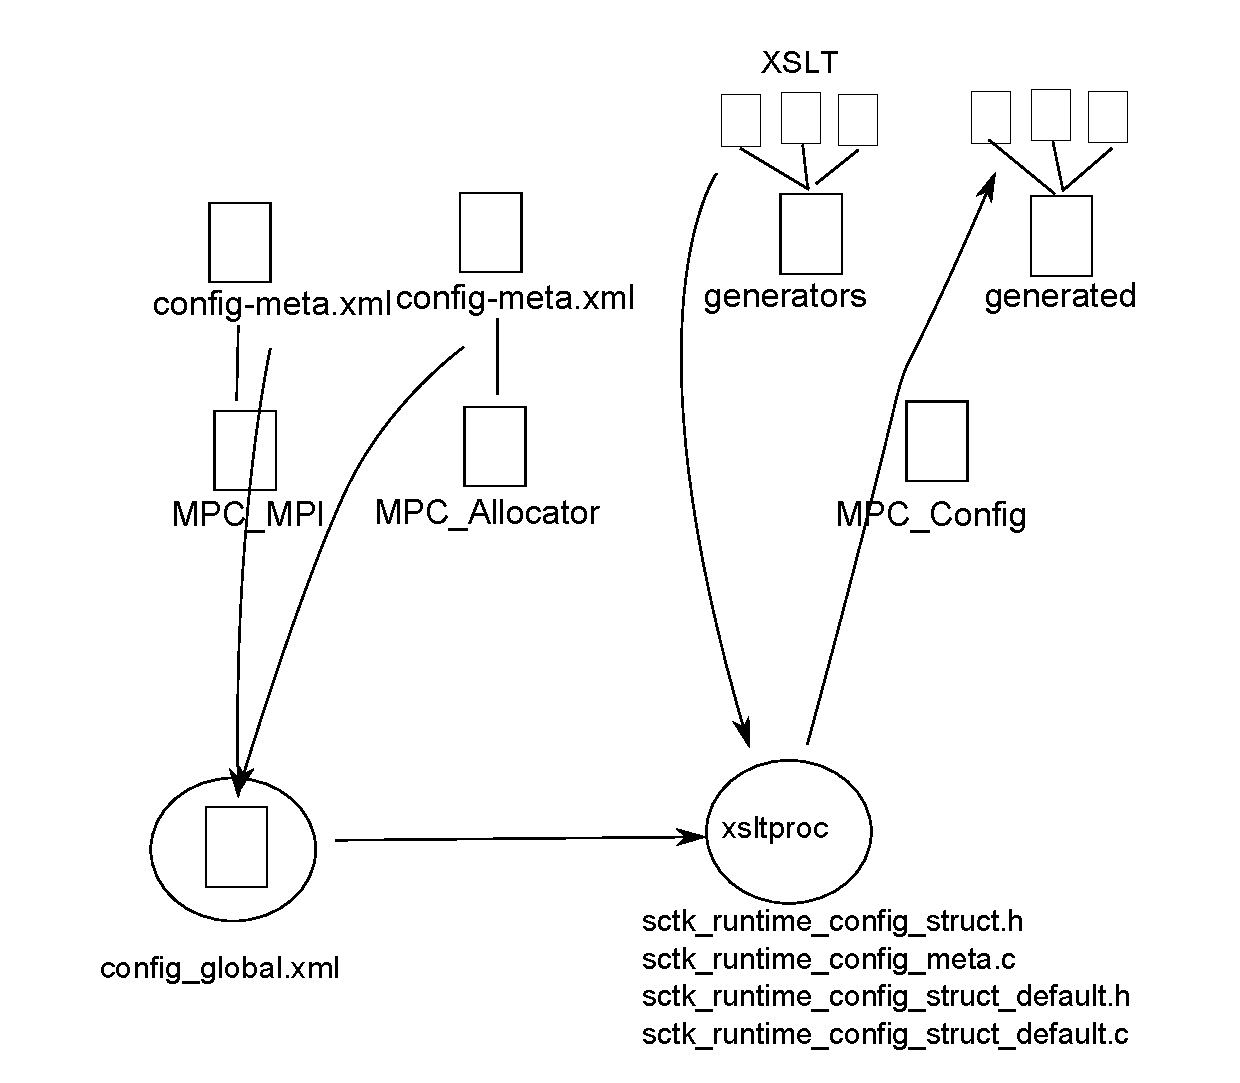
\includegraphics[scale=0.8]{file-workflow.pdf}
\caption{Representation of the workflow}
\label{fig:conf_workflow_conf}
\end{figure}

\section {Steps for developper}

A developper who wants to integrate his MPC module into the configuration system must:
\begin{enumerate}
\item Create a configuration file \texttt{config-meta.xml} in his module and define all the options he wants to parametrized;
\item Mark the dependency to the MPC\_Config module by adding in the file \texttt{module\_dep}: \texttt{need\_module MPC\_Config};
\item Regenerate the MPC\_Config auto-generated files by execution \texttt{./MPC\_Tools/mpc\_gen\_runtime\_config} from \texttt{mpc} directory;
\item Include the header \texttt{sctk\_runtime\_config.h} in his source files;
\item Use the function \texttt{sctk\_runtime\_config\_get()} to access to the configuration structure.
\end{enumerate}
\end{document}
